\section*{2024.07.06 数学分析第一章保温}
\begin{enumerate}
    \item 设$\{a_n\}_{n}$是等差数列,$\{b_n\}_{n}$是等比数列。计算\begin{align*}
        &\sum_{k=1}^{n}a_k,&&\sum_{k=1}^{n}b_k,&&\sum_{k=1}^{n}a_kb_k.
    \end{align*}
    % \begin{enumerate}
    %     \item 计算\begin{equation*}
    %         \sum_{k=1}^{n}a_k
    %     \end{equation*}
    %     \item 计算\begin{equation*}
    %         \sum_{k=1}^{n}b_k.
    %     \end{equation*}
    %     \item 仿照上一问的办法来算$\sum_{k=1}^{n}a_kb_k$。\\
    %     \item 你还有其他办法计算$\sum_{k=1}^{n}a_kb_k$吗?
    % \end{enumerate}
    \item 设$\{a_n\}_{n=1}^\infty$是实数列,$a$是一个实数。证明下述两条的等价性。
    \begin{enumerate}
        \item $\forall \varepsilon>0, \exists N\in \positiveinteger, \forall n>N, |a_n-a|<\varepsilon$.
        \item $\forall \varepsilon>0, \exists N\in \positiveinteger, \forall n>N, |a_n-a|<\varepsilon/2$.
    \end{enumerate}
    \item 说明下述数列的单调性。
    \begin{align*}
        &\left\{\Bigl(1+\frac{1}{n}\Bigr)^n\right\}_{n=1}^\infty, && \left\{\Bigl(1+\frac{1}{n}\Bigr)^{n+1}\right\}_{n=1}^\infty, && \left\{\sum_{k=0}^{n}\frac{1}{k!}\right\}_{n=0}^\infty.
    \end{align*}
    当$n$取相同值时,上述三个数列相应项的大小关系如何?
    \item 证明实数列的Cauchy收敛准则。
    \item \begin{enumerate}
        \item 给出排列数和组合数的排列组合解释,并分别说明其计算公式。
        % \item 只用一个组合数来表达$\binom{n-1}{m-1}+\binom{n-1}{m}.$
        \item 写出$(1+x)^n$的二项展开式,其中$x$取实值。
        \item 计算\begin{align*}
                &\sum_{0\leqslant k\leqslant n} \binom{n}{k},&&\sum_{\begin{subarray}{c} 0\leqslant k\leqslant n\\2\mid k\end{subarray}} \binom{n}{k},&&\sum_{\begin{subarray}{c}0\leqslant k\leqslant n\\2\nmid k\end{subarray}} \binom{n}{k}.
            \end{align*}提示:可适当利用上一问的结果。
        \item 将上述二项展开式按$x$的升幂排列,并将系数排成杨辉三角(Pascal三角),如图~\ref{图:杨辉三角}~所示。对于$n\in \positiveinteger$, 第$n+1$行为$(1+x)^{n-1}$的系数。
        \begin{figure}
            \centering
            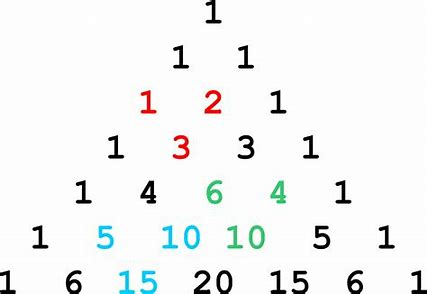
\includegraphics[scale=.5]{sections/杨辉三角.jpg}
            \caption{杨辉三角(Pascal三角)}
            \label{图:杨辉三角}
        \end{figure}
        杨辉三角是左右对称的,这体现了组合数的什么规律?
        \item 分别观察杨辉三角中的红色、绿色、蓝色数字,它们体现了组合数的什么性质?
        \item 对于固定的$n\in \positiveinteger$, 观察、猜想并证明有限长的组合数序列$\left\{\binom{k}{n}\right\}_{k=0}^n$的增减性规律。
    \end{enumerate}
    \item 写出立方差公式。
    \item \begin{enumerate}
        \item 设$E$是$\realset$的一个非空子集。证明:或者$\inf E\in E$, 或者存在严格减序列$\{a_n\}_{n=1}^\infty\subseteq E$满足$\lim_{n\to\infty}a_n=\inf E$, 这二者总是至少有一个成立。
        \item 证明自然数集的任何非空子集都有最小值。
    \end{enumerate}
    \item 设$a\in \realset$. 证明:数列$\{a_n\}_{n=1}^\infty$收敛到$a$当且仅当它的上下极限都是$a$.
    \item 设有数列$\{a_n\}_{n=1}^\infty\subset \realset,\{b_n\}_{n=1}^\infty\subset [0,\infty)$, 且$a^*:=\limsup_{n\to \infty}a_n\in \realset$, $\{b_n\}_{n=1}^\infty$收敛到一个有限实数$b$. 证明\begin{equation*}
        \limsup_{n\to\infty} a_nb_n=a^*b.
    \end{equation*}
    \item 说明Cauchy命题的逆命题一般不成立,即对于实数列$\{a_n\}_{n=1}^\infty$, 不能从$\lim_{n\to\infty}\frac{1}{n}\sum_{k=1}^{n}a_k=a\in [-\infty,+\infty]$推知$\lim_{n\to\infty}a_n=a$.
    \item 设有实数列$\{a_n\}_{n=1}^\infty$. 比较下面四式的大小关系并证明。\begin{align*}
        &\liminf_{n\to\infty}a_n,
        &&\limsup_{n\to\infty}a_n,
        &&\liminf_{n\to\infty}\frac{1}{n}\sum_{k=1}^{n}a_k,
        &&\limsup_{n\to\infty}\frac{1}{n}\sum_{k=1}^{n}a_k.
    \end{align*}
    \item 设实数列$\{a_n\}_{n=1}^{\infty}$的每一项都大于0. 比较下面四式的大小关系并证明。\begin{align*}
        &\liminf_{n\to\infty}\sqrt[n]{a_n},&&\limsup_{n\to\infty}\sqrt[n]{a_n},&&\liminf_{n\to\infty}\frac{a_{n+1}}{a_n},&&\limsup_{n\to\infty}\frac{a_{n+1}}{a_n}.
    \end{align*}
\end{enumerate}